\documentclass{beamer}

\usepackage[utf8]{inputenc}
\usepackage{tikz}
\usepackage{csquotes}
\usepackage{gnuplottex} % [noshell]: do not regenerate gnuplots
\usepackage{booktabs}
\usepackage{listings}
\lstset{
  language=python,
  basicstyle=\scriptsize,
}
\usetheme{ODK}
\usefonttheme[onlymath]{serif}
\usepackage{xspace}
\newenvironment{smatrix}{\left[\begin{smallmatrix}}{\end{smallmatrix}\right]}
\newcommand{\Z}{\ensuremath{\mathbb{Z}\xspace}}
\newcommand{\Q}{\ensuremath{\mathbb{Q}\xspace}}
\newcommand{\F}{\ensuremath{\mathbb{F}\xspace}}
\AtBeginSection[]
{
  \begin{frame}<beamer>
    \frametitle{Outline}
    \tableofcontents[currentsection]
  \end{frame}
}

\title[WP 5]{Workpackage 5:\\ High Performance Mathematical Computing}

\author[V. Delecroix, A Konovalov, C. Pernet]{Vincent Delecroix, \\ Alexander Konovalov,\\ Clément Pernet, }

\date[Luxembourg, 30/10/18]{Luxembourg, October 30, 2018}

\institute[ODK 2nd project review]{Second OpenDreamKit Project review}

\begin{document}
\maketitle

%%%%%%%%%%%%%%%%%%%%%%%%%%%%%%%%%%%%%%%
\section*{Introduction}

\begin{frame}
  \frametitle{High performance mathematical computing}

  \begin{block}{Mathematical computing}

    %% \begin{columns}
    %%   \begin{column}{.5\textwidth}
    Computing with a large variety of objects
        \begin{itemize}[<+->]
        \item $\Z, \Q, \Z/p\Z, \F_q$, \hfill {\color{blue} $17541718814389012164632$}
        \item Polynomials over $\Z, \Q, \Z/p\Z, \F_q$, \hfill {\color{blue} $\frac{2}{5} x^{3} + x^{2} - \frac{1}{19} x + 2$}
        \item Matrices over $\Z, \Q, \Z/p\Z, \F_q$, \hfill
           {\color{blue} $\begin{smatrix} 27&3&-1\\ 9&0& 2 \end{smatrix} $}
        \item Matrices of polynomials over $\Z, \Q, \Z/p\Z, \F_q$, \hfill
          {\color{blue} $ \begin{smatrix}
            3 x^{2} + 3 & 2 x^{2} + 3 \\4 x^{2} + 1 & x^{2} + 4 x + 4
          \end{smatrix}$}
        \item Tree algebra \hfill
      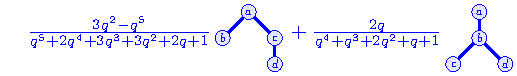
\includegraphics[width=.7\textwidth]{Pictures/operade}
        \end{itemize}
    %%   \end{column}
    %%   \begin{column}{.45\textwidth}
    %%   \end{column}
    %% \end{columns}

        for applications where all digits matter.

  \end{block}
\end{frame}

\begin{frame}
  \frametitle{High performance mathematical computing}
%  \begin{block}
  \textbf{Need for High performance:} applications where size matters:
    \begin{description}
    \item[Experimental maths:] testing conjectures
      \begin{itemize}
      \item larger instances give higher confidence
      \end{itemize}
    \item<2->[Algebraic cryptanalysis:] security = computational difficulty
      \begin{itemize}
      \item key size determined by the largest solvable problem
        \begin{columns}
          \begin{column}
            {.1\textwidth}
          \end{column}
          \begin{column}
            {.85\textwidth}
        \begin{example}
        {\small Breaking RSA by integer factorization: $n=pq$}.   Last record:
        \begin{itemize}
        \item $n$ of 768 bits
        \item linear algebra in dimension $192\,796\,550$ over $\mathbb{F}_2$ (105Gb)
        \item About 2000 CPU years
        \end{itemize}
      \end{example}
          \end{column}
        \end{columns}
      \end{itemize}
    \item<3->[3D data analysis, shape recognition:] \
      \begin{itemize}
      \item via persistent homology
      \item large sparse matrices over $\F_2$, \Z
      \end{itemize}
    \end{description}
    
    
    %% \begin{itemize}
    %% \item Decades of development for numerical computations
    %% \item Still at an early development stage for computer algebra
    %% \item Specificites: cannot blindly benefit from numerical HPC experience
    %% \end{itemize}
% \end{block}
\end{frame}
%%%%%%%%%%%%%%%%%%%%%%%%%%%%%%%%%%%%%%%%%%%%%%%%%%%%%%%%%%%%%%%%%
\begin{frame}
  \frametitle{Goal: delivering high performance to maths users}

\uncover<2->{
  \only<1,2>{
    \begin{block}{Harnessing modern hardware $\leadsto$ parallelisation}
  \begin{itemize}
    \item in-core parallelism (SIMD vectorisation)
    \item multi-core parallelism
    \item distributed computing: clusters, cloud
    \end{itemize}
  \end{block}
  }
  
  \only<3>{
    \begin{block}{Languages}
    \begin{itemize}
    \item Computational Maths software uses high level languages (e.g. Python)
    \item High performance delivered by languages close to the metal (C, assembly)
    \end{itemize}
    $\leadsto$ compilation,  automated optimisation
  \end{block}
    \vspace{.5mm}
  }
}


  \begin{center}

    \only<1>{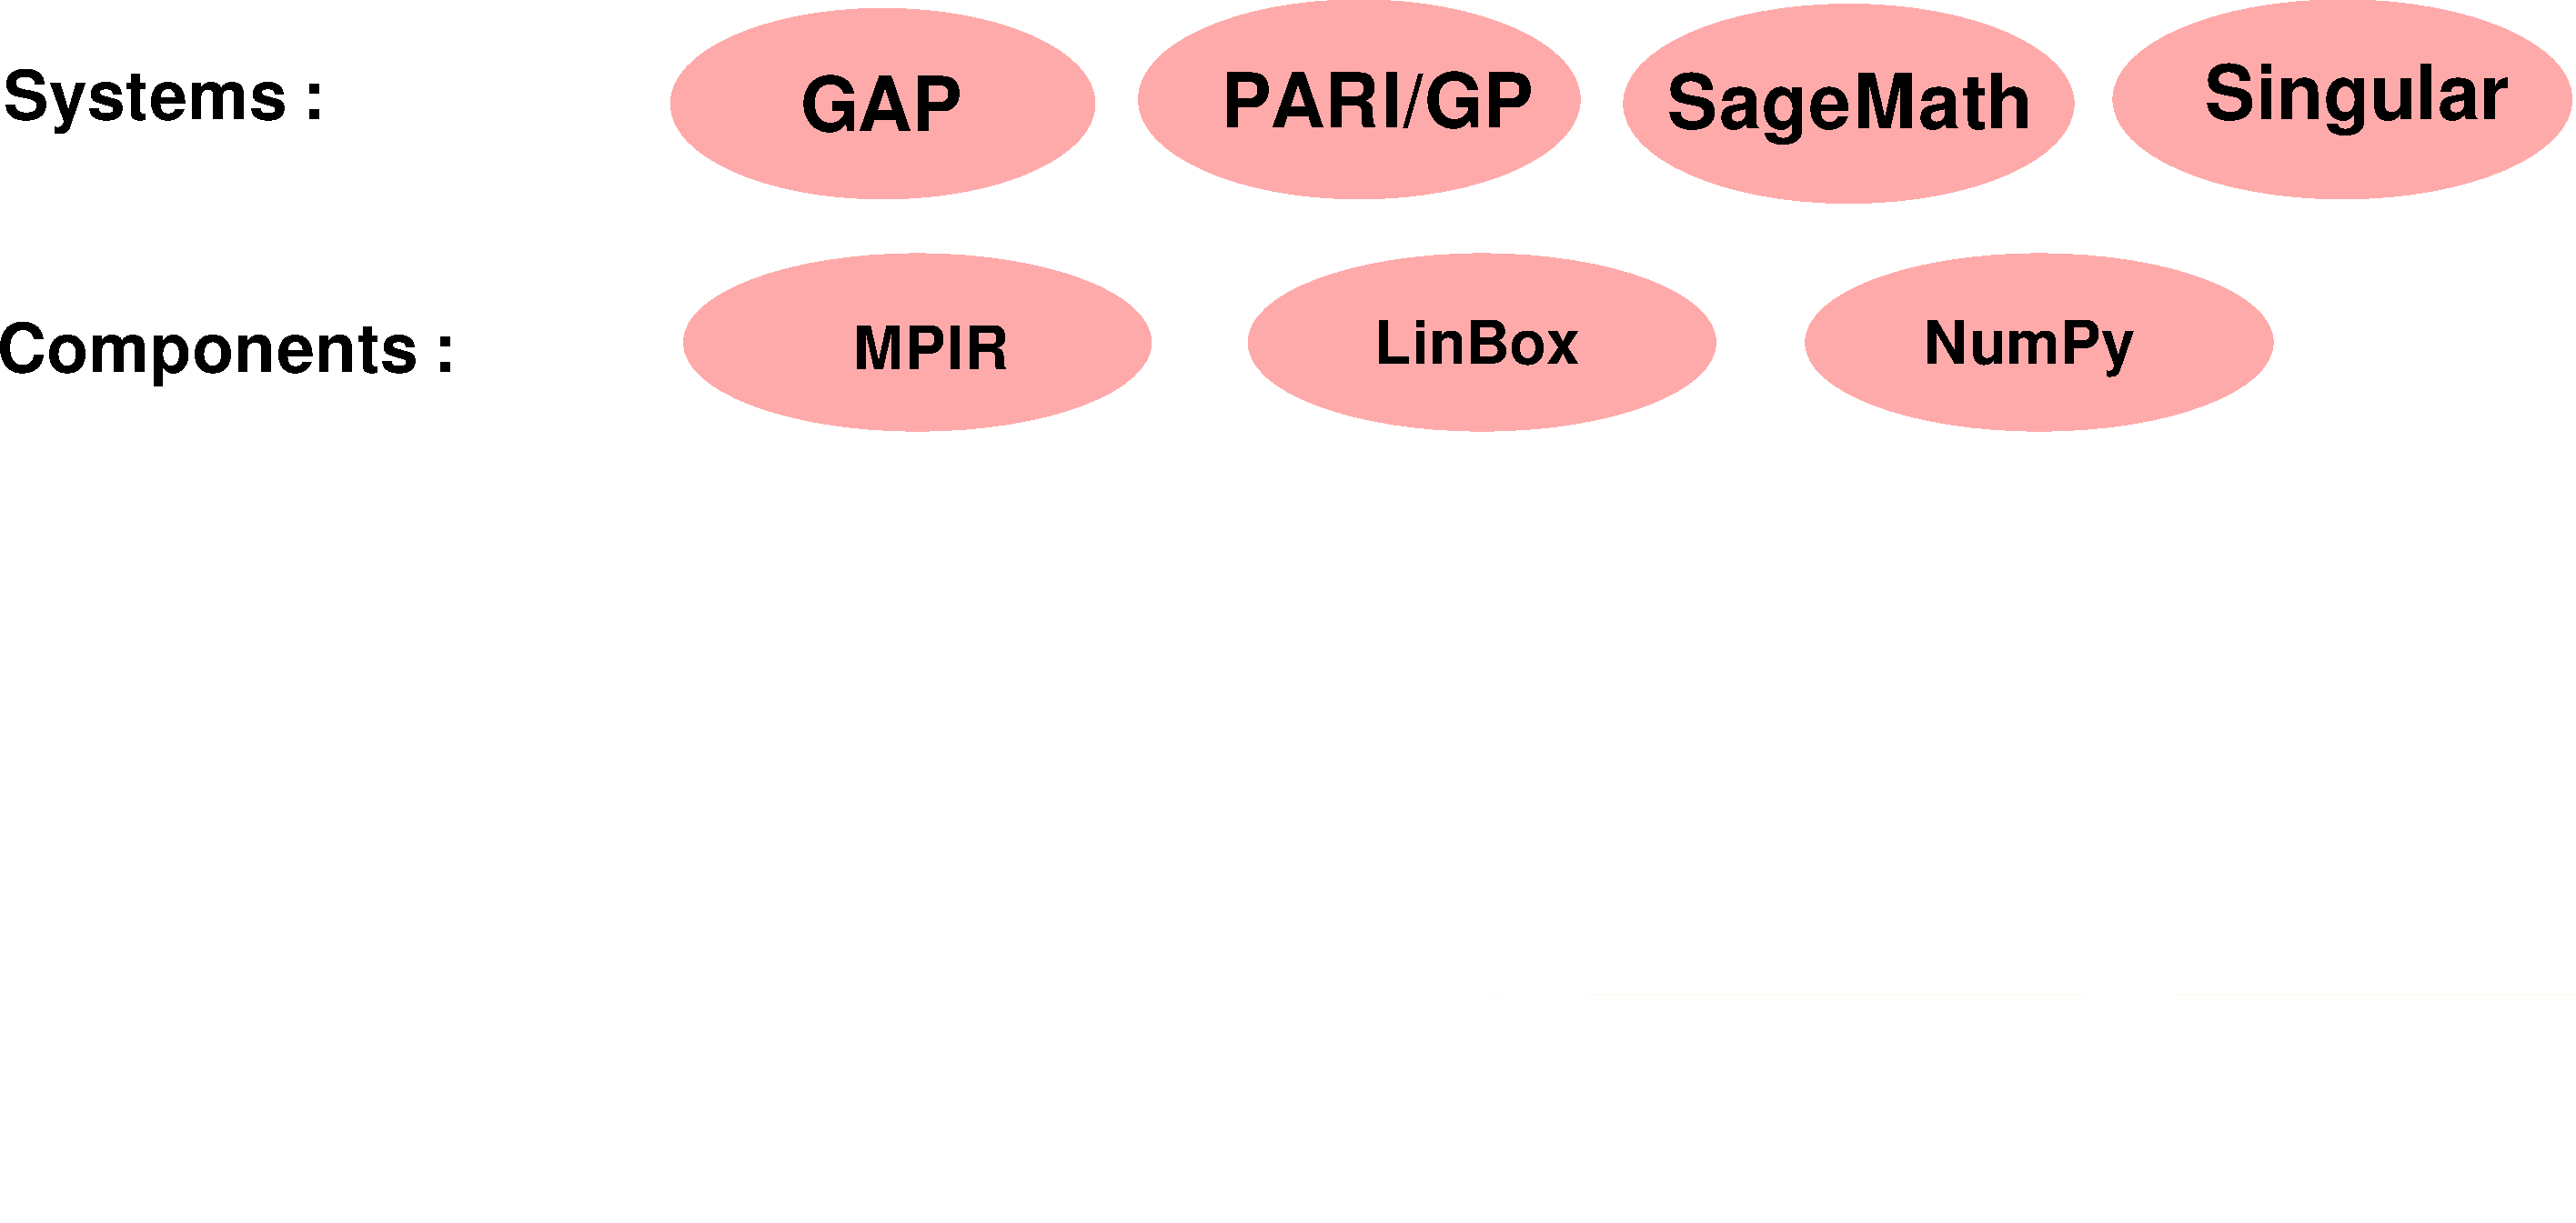
\includegraphics[width=0.8\textwidth]{software_stack_3}}

    \only<2>{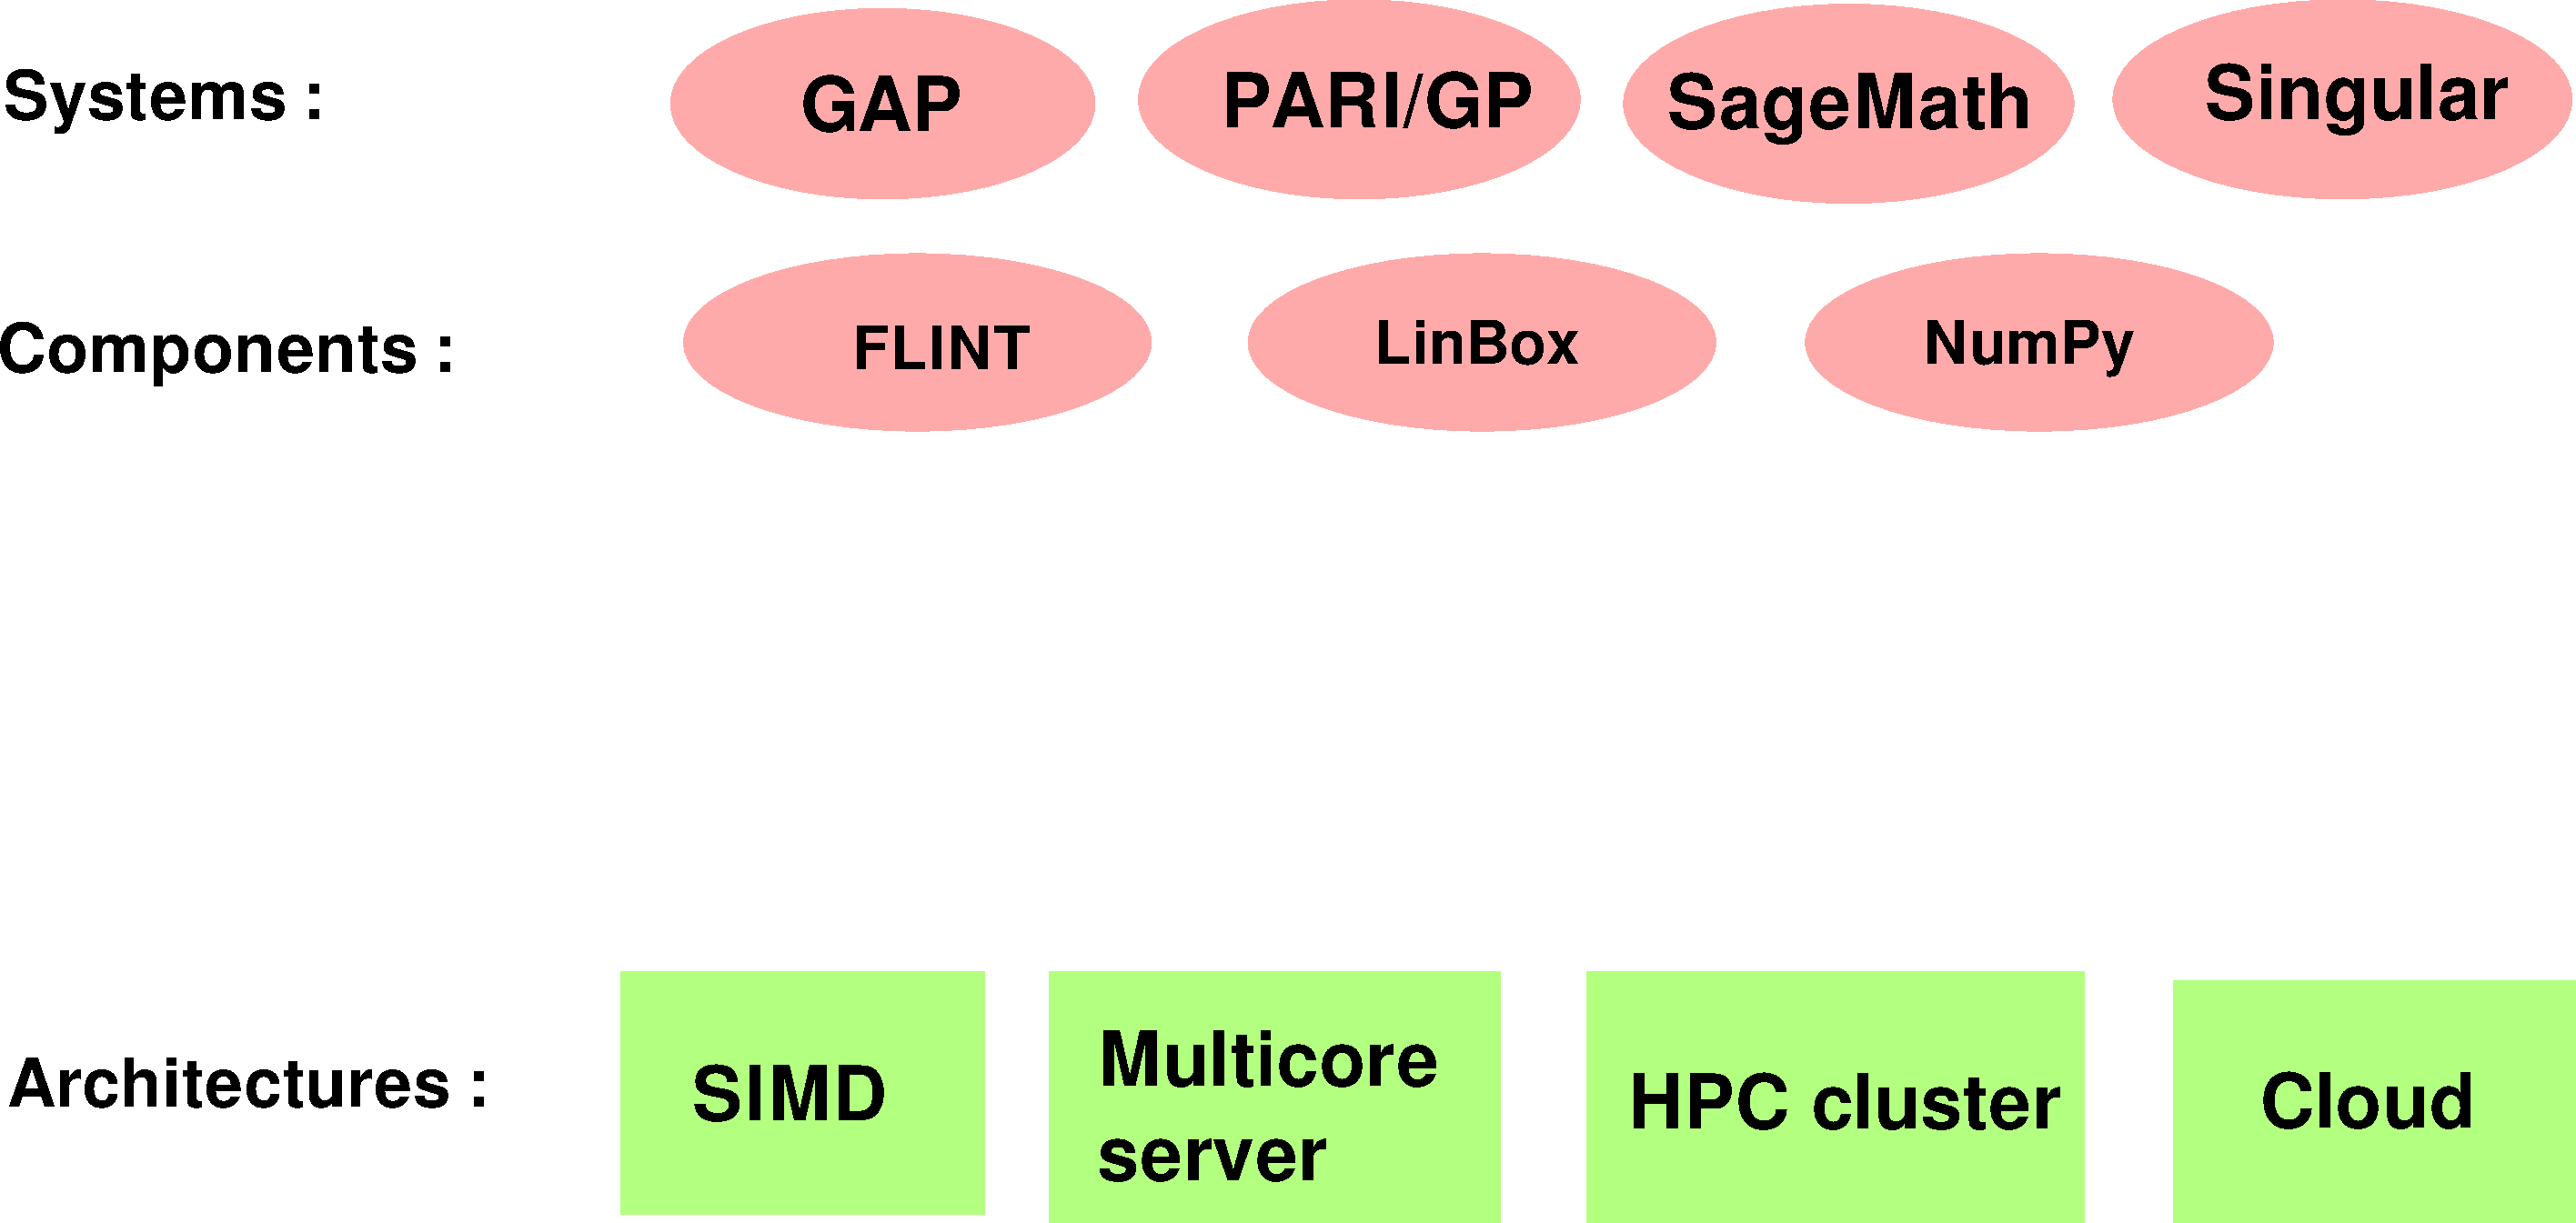
\includegraphics[width=0.8\textwidth]{software_stack_2}}
    
    \only<3>{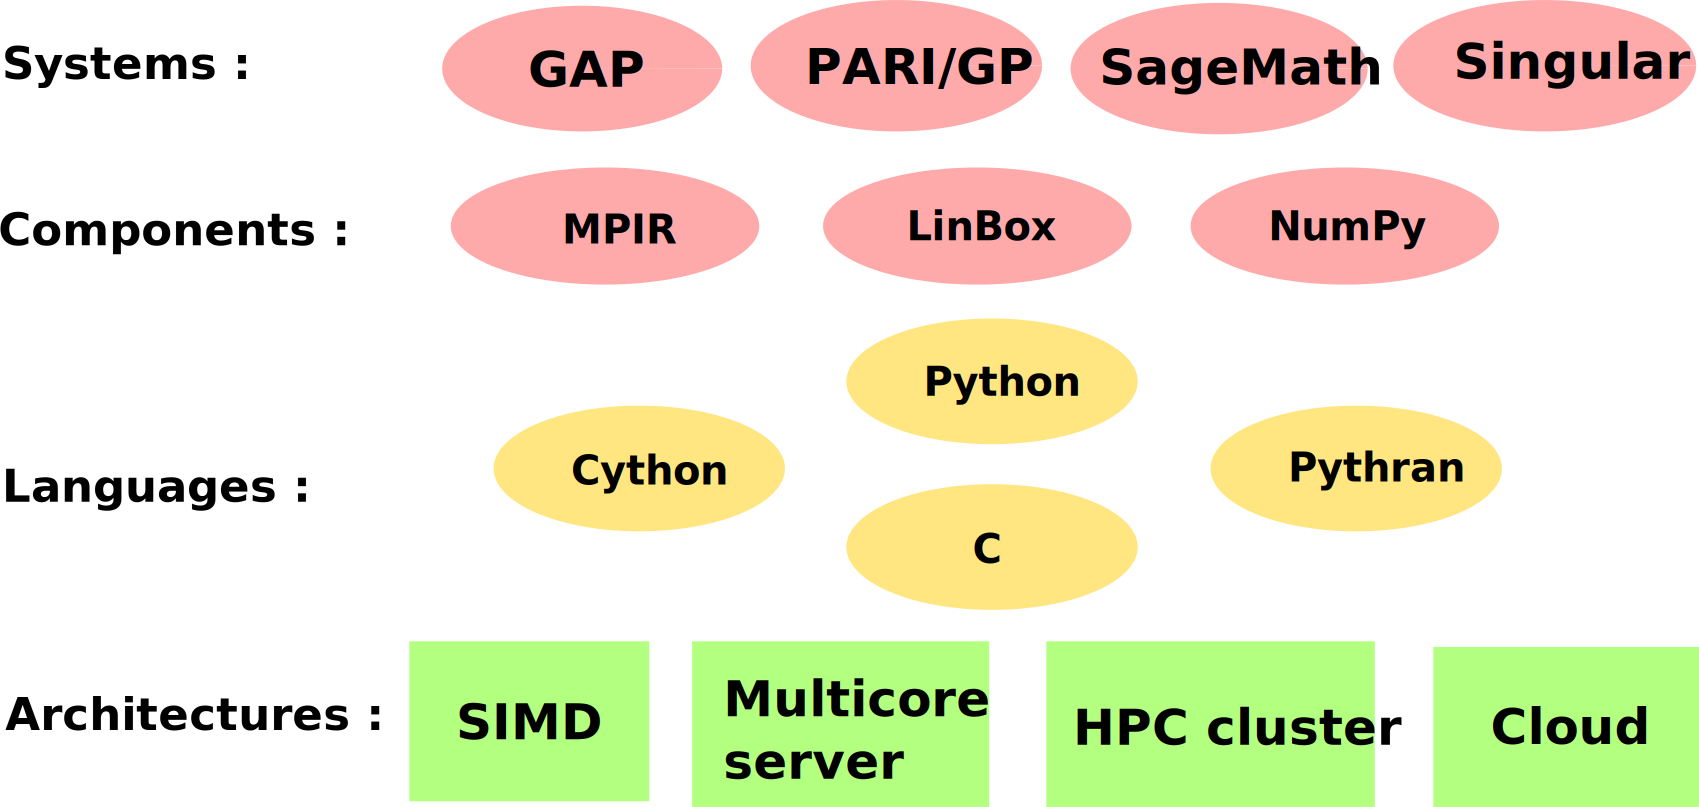
\includegraphics[width=0.8\textwidth]{software_stack}}

  \end{center}

\end{frame}
%%%%%%%%%%%%%%%%%%%%%%%%%%%%%%%%%%%%%%%%%%%%%%%%%%%%%%%%%
%% \begin{frame}
%%   \frametitle{Goal: delivering high performance to maths users}

%%     \begin{center}
%%     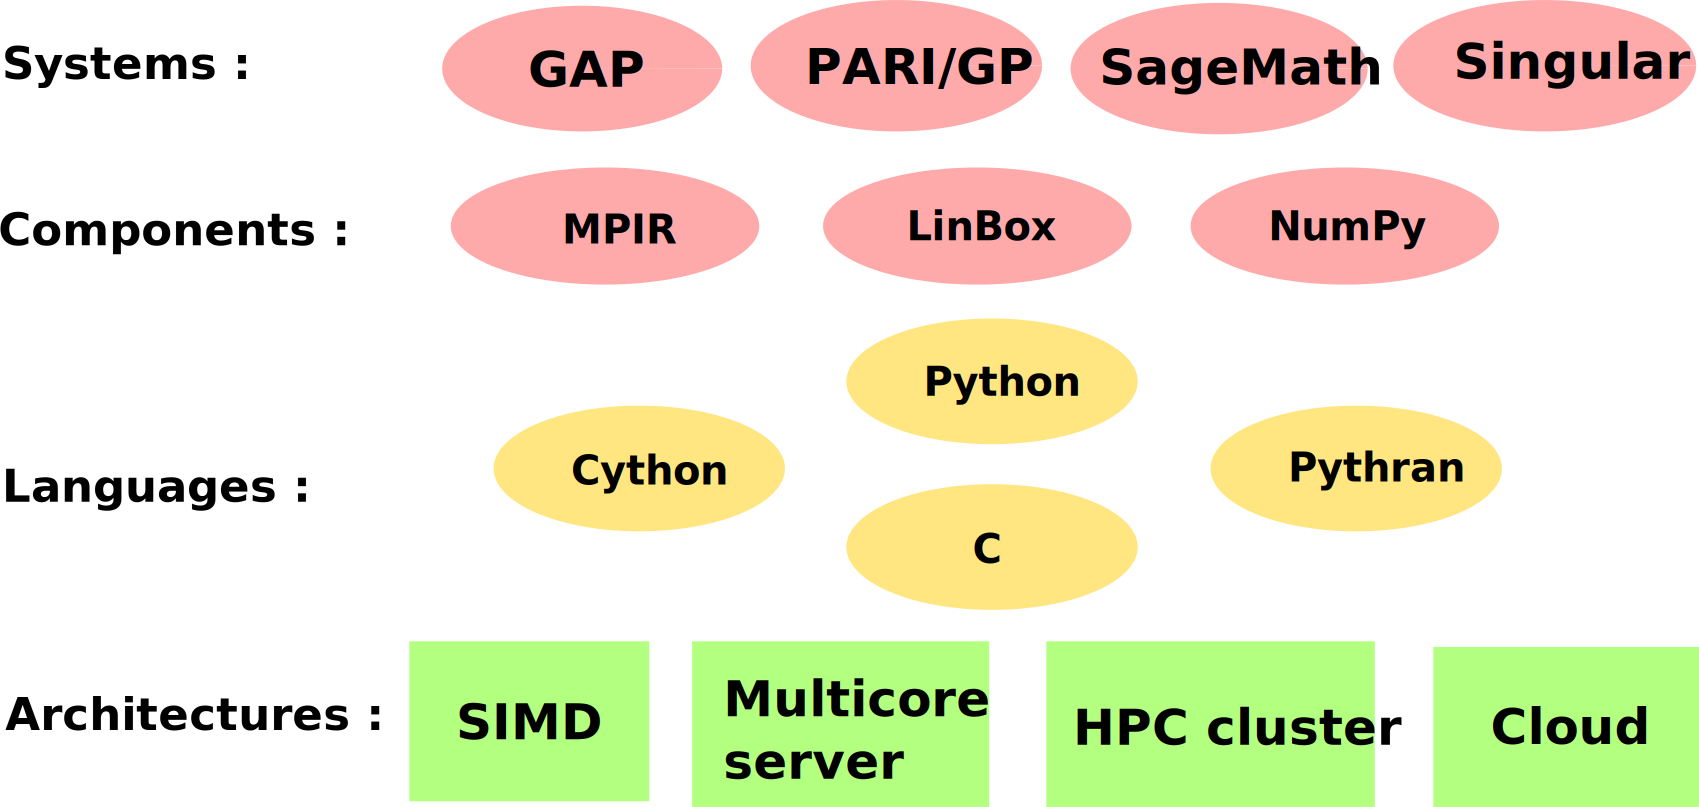
\includegraphics[width=0.8\textwidth]{software_stack}
%%   \end{center}

%%     \pause
%%     \begin{itemize}
%%     \item Improve/Develop parallel features of components first,
%%     \item Expose them through the software stack
%%     \item 
%%     \end{itemize}

%% \end{frame}


%%%%%%%%%%%%%%%%%%%%%%%%%%%%%%%%%%%%%%%
\begin{frame}
  \frametitle{High performance mathematical computing}
  \begin{block}
    {Goal:}
    \begin{itemize}
    \item Improve/Develop parallelization of software components
    \item Expose them through the software stack
    \item Offer High Performance Computing to VRE's users
    \end{itemize}
  \end{block}

  \begin{block}
      {Milestone M8: Seamless use of parallel computing architecture in the VRE (proof of concept)}

{\footnotesize  \textit{Astrid wants to run compute intensive routines involving both dense linear algebra and combinatorics. She has access through a JupyterHub-based VRE to a high end multi-core machine which includes a vanilla SAGE installation.
She automatically benefits from the HPC features of the underlying specialized
libraries (LinBox, ...). This is a proof of concept of the overall framework to
integrate the HPC advances of specialized libraries into a general purpose
VRE. It will prepare the final integration of a broader set of such parallel
features for the end of the project}
  }

  \end{block}
\end{frame}

%%%%%%%%%%%%%%%%%%%%%%%%%%%%%%%%%%%%%%%%%%%%%%%%%%%%%%

%% \begin{frame}[fragile]
%%   \frametitle{Milestone M8: Seamless use of parallel computing architecture in the VRE (proof of concept)}

%%   \begin{center}
%%     Live demo
%%   \end{center}
%% \end{frame}
%%%%%%%%%%%%%%%%%%%%%%%%%%%%%%%%%%%%%%%%%%%%%%%%%%%%%%
%%%%%%%%%%%%%%%%%%%%%%%%%%%%%%%%%%%%%%%
\begin{frame}
  {Outline}
  \tableofcontents
\end{frame}

%%%%%%%%%%%%%%%%%%%%%%%%%%%%%%%%%%%%%%%
%%%%%%%%%%%%%%%%%%%%%%%%%%%%%%%%%%%%%%%
\section{Workpackage management}
\begin{frame}
  \frametitle{Outcome of WorkPackage 5}

  \begin{tabular}{lccc}
    \toprule
    Component & Review 1 & Review 2 & Final review\\
    \midrule
    T5.1 Pari/GP & & & {\color{green} D5.16} \\
    T5.2 GAP     & & & {\color{green} D5.15} \\
    T5.3 LinBox  & & \alert{D5.12} & {\color{green} D5.14} \\
    T5.4 Singular& D5.6, D5.7 & & {\color{green} D5.13} \\
    T5.5 MPIR    & D5.5, D5.7& & \\
    T5.6 Combinatorics  & D5.1& \alert{D5.11} & \\
    T5.7 Pythran        & D5.2 & \alert{D5.11} & \\
    T5.8 SunGrid Engine & D5.3 & & \\
    \bottomrule
    
  \end{tabular}

  \vspace{1em}
  
  Overall
  \begin{itemize}
  \item over 20 software relases were cut
  \item 7 research papers
  \end{itemize}
\end{frame}

%%%%%%%%%%%%%%%%%%%%%%%%%%%%%%%%%%%%%%%%%%%%%%%%%%%%%%
\begin{frame}
\frametitle{Addressing recommendations of review 1}
    \textbf{Recommendation 10:} \textit{Regarding WP5, \textbf{make contacts} with HPC community in order to ascertain current state-of-the-art. The work in this WP needs to be \textbf{nearer the leading edge}.}

    \begin{description}
    \item<2-> [Leading edge achievements in linear algebra] \
      {\small
      \begin{itemize}
      \item symmetric factorization outperforms LAPACK implementation
      \item new non-hierarchical generator for quasiseparable matrices
      \item large scale parallelization of rational linear solver
      \end{itemize}
      }
    \begin{columns}
      \begin{column} {.3\textwidth}
        \begin{center}
          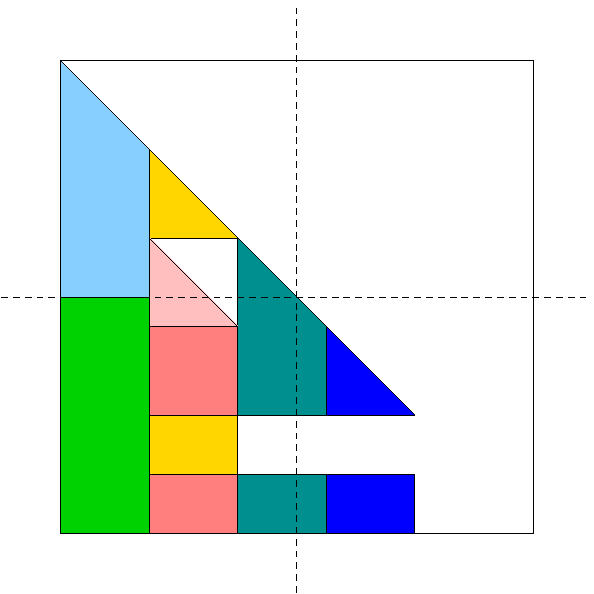
\includegraphics[width=.6\textwidth]{ARrec11}
      \end{center}
      \end{column}
      \begin{column} {.3\textwidth}
        \begin{center}
          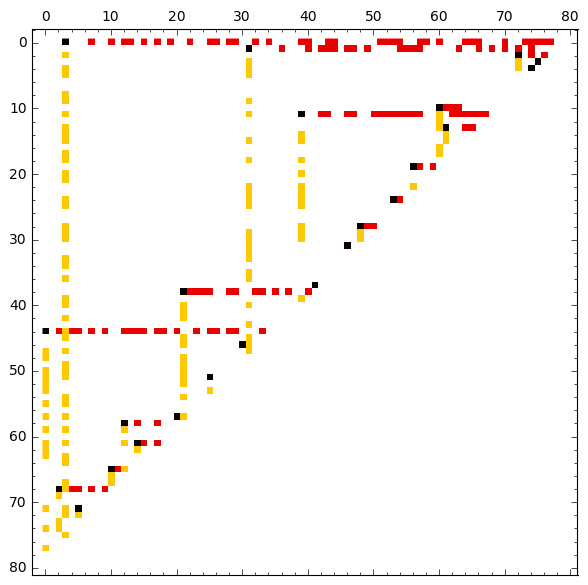
\includegraphics[width=.6\textwidth]{Bruhat}
        \end{center}
      \end{column}
      \begin{column} {.3\textwidth}
        \begin{center}
          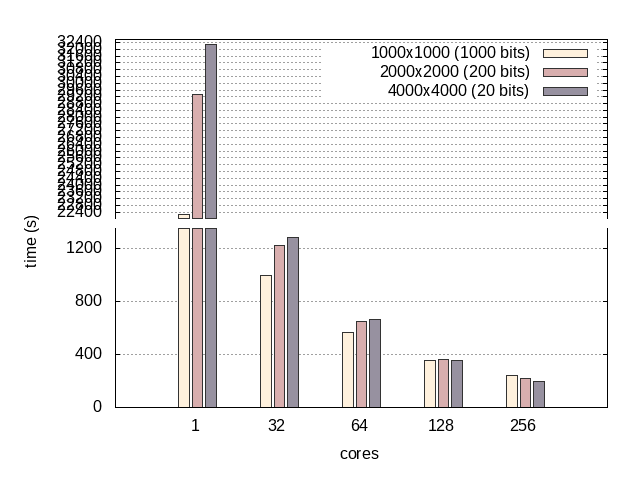
\includegraphics[width=.9\textwidth]{nodes_histogram}
        \end{center}
      \end{column}
    \end{columns}
    %% \item<3-> [Interactions and  contacts made:]\ 
    %%   {\small
    %%   \begin{itemize}
    %%   \item interaction with the \texttt{BLIS} group (vectorization and
    %%     implementation of Strassen's algorithm)
    %%   \item on-going collaboration with T. Mary (\texttt{Mumps}) and
    %%     S. Chandrasekaran (UCSB) on quasiseparable matrix algorithmic
    %%   \end{itemize}
    %%   }
\end{description}
\end{frame}


%%%%%%%%%%%%%%%%%%%%%%%%%%%%%%%%%%%%%%%
% TODO: should this be the same title as the one above
% "Addressing recommendations of review 1"
\begin{frame}
  \frametitle{Strengthening interactions with numerical HPC community}
  \begin{block}  {Existing connection}
    \begin{description}
    \item[Dense linear algebra] numerical BLAS used for exact FFLAS for 17 years
    \item[Pointwise interactions:] J. Dongarra, L. Grigori, J-Y. L'Excellent,  etc
    \item[Publications to in main HPC venues:]
      SIAM-PPSC, EuroPar, PMAA, ParCo
    \item[Animation:] involved in the French CNRS \textit{Calcul}  working group (Sci. Comp.)
    \end{description}
  \end{block}
  \begin{block}<2->  {Recently established}
    \begin{itemize}
    \item With the \texttt{BLIS} group:
      \begin{itemize}
      \item Reporting bugs (SIMD vectorization)
      \item Sharing experience in implementing Strassen's algorithm
      \end{itemize}
    \item On-going collaboration with T. Mary (\texttt{Mumps}) and
        S. Chandrasekaran (UCSB) on quasiseparable matrix algorithmic
    \end{itemize}
  \end{block}
\end{frame}

%%%%%%%%%%%%%%%%%%%%%%%%%%%%%%%%%%%%%%%
%%%%%%%%%%%%%%%%%%%%%%%%%%%%%%%%%%%%%%%
\section{Exact linear algebra}
%%%%%%%%%%%%%%%%%%%%%%%%%%%%%%%%%%%%%%%
\subsection{Exact linear algebra algorithms and implementations (D5.12).}

\begin{frame}
  \frametitle{Task 5.3: LinBox, High performance exact linear algebra}
  \begin{displayquote}
    Mathematics is the art of reducing any problem to linear algebra\\
    \hfill{-- W. Stein}
  \end{displayquote}

\uncover<2->{  \begin{center}
  \textbf{Linear algebra: a key building block for HPC}
  \end{center}
  }
  \begin{block}<2-> {Similarities with numerical HPC}
    \begin{itemize}
    \item central elementary problem to which others reduce to
    \item (rather) simple algorithmic
    \item high compute/memory intensity
    \end{itemize}
  \end{block}
    \begin{block}<3->{Specificities}
      \begin{itemize}
      \item Multiprecision arithmetic $\Rightarrow$ lifting from finite  precision ($\mathbb{F}_p$)
      \item Rank deficiency $\Rightarrow$ unbalanced dynamic blocking
      \item Early adopter of subcubic matrix arithemtic $\Rightarrow$ recursion
      \end{itemize}
    \end{block}
      
    \end{frame}
%%%%%%%%%%%%%%%%%%%%%%%%%%%%%%%%%%%%%%%%%%%%%%%ù
\begin{frame}
  \frametitle{D5.12: Exact linear algebra algorithms and implementations. Library maintenance and close integration in mathematical software for LinBox library}

  \begin{enumerate}
  \item Algorithmic innovations:
    \begin{enumerate}
    \item Rank deficient dense Gaussian elimination
    \item Quasiseparable matrices
    \item Outsourced computing security
    \end{enumerate}
  \item Software releases and integration:
    \begin{enumerate}
    \item LinBox ecosystem: \texttt{LinBox, fflas-ffpack, givaro}
    \item \texttt{SageMath} integration
    \end{enumerate}
  \end{enumerate}
\end{frame}

%%%%%%%%%%%%%%%%%%%%%%%%%%%%%%%%%%%%%%%
\begin{frame}
  \frametitle{Rank deficient dense Gaussian elimination}
%%   \begin{block}
%%     {[JSC'17] Fast computation of the rank profile matrix and the generalized
%%       Bruhat decomposition.}
%% {    \small
%%   \begin{itemize}
%%     \item Connecting Rank Profile Matrix and row and column echelon forms
%%     \item $O\tilde\ (r^\omega + mn)$ probabilistic time
%%     \item generalization over arbitrary rings
%%     \end{itemize}
%% }
%%   \end{block}

  \begin{block}{[ISSAC'18] Symmetric triangular factorization}
    \begin{columns}
      \begin{column} {.65\textwidth}
        \begin{itemize}
        \item First unconditional recursive algorithm
        \item Pivoting revealing the Rank Profile Matrix
        \item $O(n^2r^{\omega-2}) $ ($=1/3n^3$ with $\omega=3, r=n$)
        \item Also hot topic in numerical linalg \\ [LAPACK Working notes 294, Dec'17]
        \end{itemize}
      \end{column}
      \begin{column} {.25\textwidth}
        \begin{center}
          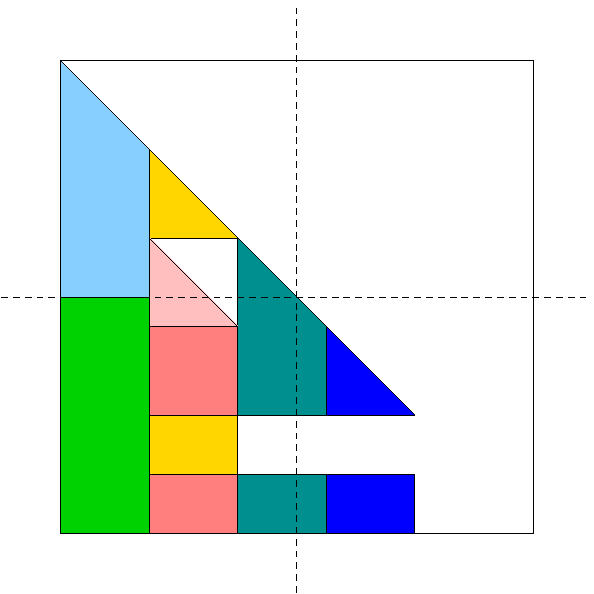
\includegraphics[width=\textwidth]{ARrec11}
        \end{center}
      \end{column}
    \end{columns}
  \end{block}
\end{frame}

%%%%%%%%%%%%%%%%%%%%%%%%%%%%%%%%%%%%%%%%%%%%%%%%%%%%%%%%%%%%%%%  
\begin{frame}[fragile]
\frametitle{LAPACK vs FFPACK modulo $8\,388\,593$}

{\footnotesize
  \begin{center}
\begin{tabular}{rrrrr}
\toprule
& \multicolumn{2}{c}{LAPACK}&\multicolumn{2}{c}{FFPACK}\\
$n$ & dgetrf (LU)  & dsytrf (LDLT) & fgetrf (LU)& fsytrf (LDLT)\\
\midrule
5000 &  2.01s & 1.60s  & 3.90s& \alert{1.59s} \\
10000 &  14.95s & 11.98s  & 24.12s& \alert{10.90s} \\
\bottomrule
\end{tabular}
\end{center}
}
%\vspace{-5pt}
%\hspace{-20pt}
%\begin{minipage}{\textwidth}
\scriptsize
%\onslide+<2>
\begin{center}
  \begin{gnuplot}[terminal=cairolatex,terminaloptions={font ",10" linewidth 2}]
  set style line 3 pt 3 pi 50 lw 4 lt rgb "blue"
  set title 'Full rank, 1-core Intel Haswell i5-4690, \symbol{64}3.5GHz' offset 0,-0.75
  set ylabel 'Effective Gfops' offset 1,0
  set xlabel 'matrix dimension' offset 0,0.1
  set xtics rotate by 30 offset -2,-0.75
  set y2tics autofreq 
  set autoscale y2fixmin
  set autoscale y2fixmax  
  set size 0.8,0.75
  set key bottom right Left reverse
  plot [1:10000] [1:45] \
  "data_gflops.txt" using 1:2 title "LAPACK dgetrf" with lines lw 4 lc 1, \ 
  "data_gflops.txt" using 1:3 title "LAPACK dsytrf" with lines lw 4 lc 2, \
  "data_gflops.txt" using 1:6 title "FFPACK fgetrf" with lines lw 4 lc 4, \
  "data_gflops.txt" using 1:7 title "FFPACK fsytrf" with lines ls 3
\end{gnuplot}
\end{center}
%\end{minipage}
\end{frame}
%%%%%%%%%%%%%%%%%%%%%%%%%%%%%%%%%%%%%%%
\begin{frame}
  \frametitle{Quasiseparable matrices }
  \begin{center}
    \textit{Matrices with low off-diagonal rank}
  \end{center}

  \begin{block}
    {[ISSAC'16, JSC'18] New compact representation and algorithms}
  \begin{columns}
    \begin{column}{.75\textwidth}
    \begin{itemize}
    %\item Connection with rank profile matrix
    \item Matches the best space complexities%: $O(ns)$
    \item Reduction to matrix multiplication%: $O(ns^{\omega-1})$ for products
    \item \textbf{Breakthrough:} Flat representation (non hierarchical)
    \end{itemize}
    \uncover<2->{
      \begin{description}
      \item[Follow-up:] on-going collaboration with numerical HPC experts:
        \begin{itemize}
        \item S. Chandrasekaran (UCSB)
        \item T. Mary (U. Manchester, \texttt{Mumps})
        \end{itemize}
      \end{description}
      }
    \end{column}
    \begin{column}{.2\textwidth}
      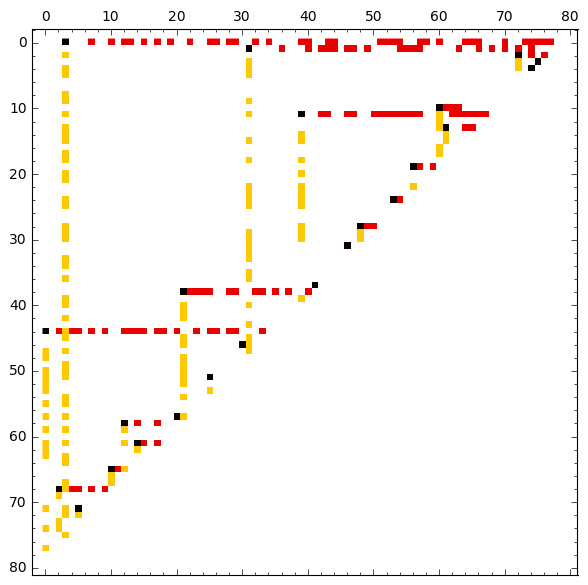
\includegraphics[width=\textwidth]{Bruhat}
    \end{column}
  \end{columns}
  \end{block}

\end{frame}


%%%%%%%%%%%%%%%%%%%%%%%%%%%%%%%%%%%%%%%
%%%%%%%%%%%%%%%%%%%%%%%%%%%%%%%%%%%%%%%%%%%%%%%%%%%%%%%%
\begin{frame}{Software releases and integration}
    \begin{block} {LinBox ecosystem}
      \begin{description}
        \item[\texttt{givaro}:] field/ring arithmetic
          \hfill{\uncover<2->{\alert{4 releases}}}
        \item[\texttt{fflas-ffpack}:] dense linear algebra over finite field \hfill{\uncover<2->{\alert{6 releases}}}
        \item[\texttt{LinBox}:] exact linear algebra \hfill{\uncover<2->{\alert{6 releases}}}
      \end{description}
      Tightly integrated  in \texttt{SageMath} \hfill{\uncover<2->{\alert{13 tickets}}}
    \end{block}

    \begin{block}<3-> {Featuring}
      \begin{itemize}
      \item Full functional implementations of new algorithmic contributions
      \item Improved vectorization and parallel routines
      \item Drastic improvement of reliability (continuous integration,
        test-suite coverage, randomized certificates, etc)
      \end{itemize}
    \end{block}
\end{frame}
%%%%%%%%%%%%%%%%%%%%%%%%%%%%%%%%%%%%%%%
\subsection{Distributed computing}
\begin{frame}
  \frametitle{Distributed computing  (on-going work)}

  \begin{block} {D5.14: Distributed exact linear system solving}
{
    \only<1,2>{
      \begin{itemize}
        \item 2 full time engineers
        \item Communication and serialization layer done
        \item Prototype MPI parallelization of Chinese remainder based solver.
      \end{itemize}
    }
    \only<3->{
      \begin{description}
      \item[Roadmap:] \
        \begin{itemize}
        \item Major refactorization of LinBox solver code under way
        \item Parallelization of Dixon-lifting solver
        \item Hybrid combination of CRT+Dixon.
        \item Hyrbid OpenMP-MPI implementation
        \end{itemize}   
      \end{description}
        \vspace{-1.4em}
    }
    \begin{columns}
      \begin{column} {.5\textwidth}
        \begin{center}
          \uncover<2->{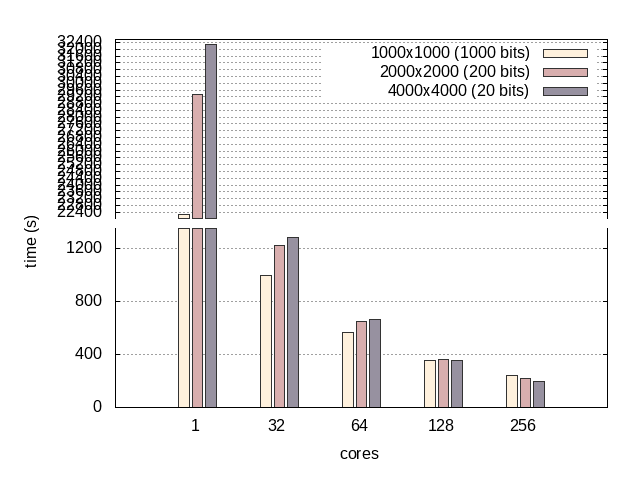
\includegraphics[width=\textwidth]{nodes_histogram}}
      \end{center}
      \end{column}
      \begin{column} {.45\textwidth}
        \begin{center}
          \uncover<2->{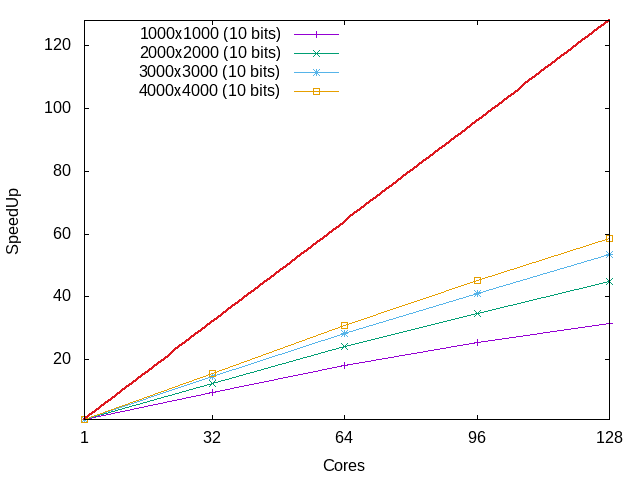
\includegraphics[width=\textwidth]{nodes_SPEEDUP}}
        \end{center}
      \end{column}
    \end{columns}
}
  \end{block}
\end{frame}

%%%%%%%%%%%%%%%%%%%%%%%%%%%%%%%%%%%%%%%%%%%%%%%%
%%%%%%%%%%%%%%%%%%%%%%%%%%%%%%%%%%%%%%%%%%%%%%%%
\section{Combinatorics}
%%%%%%%%%%%%%%%%%%%%%%%%%%%%%%%%%%%%%%%
\subsection{Refactor and optimize Sage's Combinatorics (D5.11)}
\begin{frame}
  \frametitle{Task 5.6: HPC infrastructure for Combinatorics}

  \begin{displayquote}
  \small Parallel algebraic computations exhibit high degrees of irregularity, at
  multiple levels and make no use of floating-point operations. This combination 
  means that symbolic computations are not suited to conventional HPC paradigms.
  \\ \hfill{-- P. Maier, D. Livesey, H.-W. Loidl, P. Trinder}
  \end{displayquote}

  \begin{block}{General situation}
    Given a set $S$ of combinatorial objects we want to
    \begin{itemize}
    \item find (or pick at random) an element of $S$
    \item list (or count) the elements of $S$
    \end{itemize}
  \end{block}

  \begin{block}{Specificities of combinatorics}
    \begin{itemize}
    \item \textbf{huge}: $S$ does not fit in memory
    \item \textbf{embarassingly parallel}: $S = S_1 \cup \ldots \cup S_k$
    \item \textbf{unbalanced}: $S_i$ sizes are highly unbalanced
    \end{itemize}
  \end{block}
\end{frame}
%%%%%%%%%%%%%%%%%%%%%%%%%%%%%%%%%%%%%%%
\begin{frame}
  \frametitle{D5.11: Refactor and optimise the existing combinatorics Sage code using the new developed Pythran and Cython features.}

  Algorithmic innovations and software integration through examples:
  \begin{enumerate}
  \item Example 1: polytopes
  \item Example 2: numerical semigroups
  \end{enumerate}

\end{frame}

%%%%%%%%%%%%%%%%%%%%%%%%%%%%%%%%%%%%%%%

% TODO: mettre des images ici
\begin{frame}{Example 1: polytopes (description)}
  \begin{example}
  Some combinatorial objects can be encoded as integer vectors in polytopes.
  \begin{center}
\includegraphics[scale=0.2]{Pictures/polytope.png}\end{center}
  \end{example}

   \begin{itemize}
   \item Efficient algorithms available (\emph{e.g.} Double Description, Barvinok)
   \item High performance libraries (\emph{e.g.} \texttt{PPL}, \texttt{Normaliz}, \texttt{Polymake})
   \item Useful for many combinatorial problems
   \end{itemize}
\end{frame}
%%%%%%%%%%%%%%%%%%%%%%%%%%%%%%%%%%%%%%%

\begin{frame}{Example 1: polytopes (ODK work)}
  \begin{block}{ODK outcomes}
  \begin{description}
  \item[\texttt{pplpy} library:] Python interface to the high performance
  Parma Polyhedra Library (rational polytopes)
  \hfill{\uncover<2->{\alert{6 releases}}}
  \item[\texttt{e-antic} library:] C/C++ library for computations over embedded
  number fields. Building block for multithread polytope computations in Normaliz
  over number fields.
  \hfill{\uncover<2->{\alert{release planned}}}
  \item[Workshop:] Sage Days 84
  \item[\texttt{SageMath}:] improvement of native code and libraries
  interfaces \hfill{\uncover<2->{\alert{10 tickets}}}
  \end{description}
  \end{block}

\end{frame}
%%%%%%%%%%%%%%%%%%%%%%%%%%%%%%%%%%%%%%%

\begin{frame}{Example 2: semigroups (description)}
  \begin{example}
  Numerical semigroup are certain subsets of non-negative integers.
  \begin{center}%
  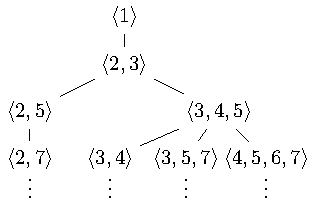
\includegraphics{Pictures/semigroups.pdf}%
  \end{center}%
  \end{example}

  \begin{itemize}
  \item Many mathematical open mathematical questions
  \item Highly unbalanced tree
  \end{itemize}
\end{frame}
%%%%%%%%%%%%%%%%%%%%%%%%%%%%%%%%%%%%%%%
\begin{frame}{Example 2: semigroups (ODK work)}

  \begin{block}{A SageMath implementation of work-stealing map-reduce}
    \begin{itemize}
    \item Work stealing algorithm (Leiserson-Blumofe)
    \item Easy to use, easy to call from SageMath with many use cases
    \item Scale well with the number of CPU cores and reasonably efficient (given that it is Python code).
    \end{itemize}
  \end{block}

  A typical speedup (parallelization of binary sequences)
  \begin{center}\begin{tabular}{c|cccc}
    \# processors & 1 & 2 & 4 & 8\\
%    Time (s) & 250 & 161 & 103 & 87
     Speedup      & $\times 1$ & $\times 1.55$ & $\times 2.43$ & $\times 2.87$
  \end{tabular}\end{center}

 \hfill{\uncover<2->{\alert{integrated in SageMath}}}
 
\end{frame}
%%%%%%%%%%%%%%%%%%%%%%%%%%%%%%%%%%%%%%%
\begin{frame}{Example 2: semigroups (ODK work)}

  \begin{block}{HPCombi: an experimental C++ library}
  \begin{itemize}
  \item innovative SIMD code for combinatorics
  \item fine grained parallelization using Intel Cilk technology
  \item already in use for mathematical projects (numerical semigroups)
  \end{itemize}
  \end{block}

  \begin{center}\begin{tabular}{l|c}
  Operation & Speedup \\\hline
  Sum of a vector of bytes & $\times 3.81$\\
  Sorting a vector of bytes& $\times 21.3$\\
  Inverting a permutation& $\times 1.97$\\
  Number of cycles of a permutation& $\times 41.5$\\
  Number of inversions of a permutation& $\times 9.39$\\
  Cycle type of a permutation& $\times 8.94$\\
  \end{tabular}\end{center}

  \hfill{\uncover<2->{\alert{Open-source library}}}

\end{frame}
%%%%%%%%%%%%%%%%%%%%%%%%%%%%%%%%%%%%%%%

%%%%%%%%%%%%%%%%%%%%%%%%%%%%%%%%%%%%%%%
%% \subsection{Task 5.7: Pythran}
%% \begin{frame}
%%   \frametitle{Task 5.7: Pythran}
%%   \begin{center}
%%     {\Large \textbf{Pythran}: a Python to C compiler}
%%   \end{center}
%%   \begin{columns}
%%     \begin{column}
%%       {.48\textwidth }
%%           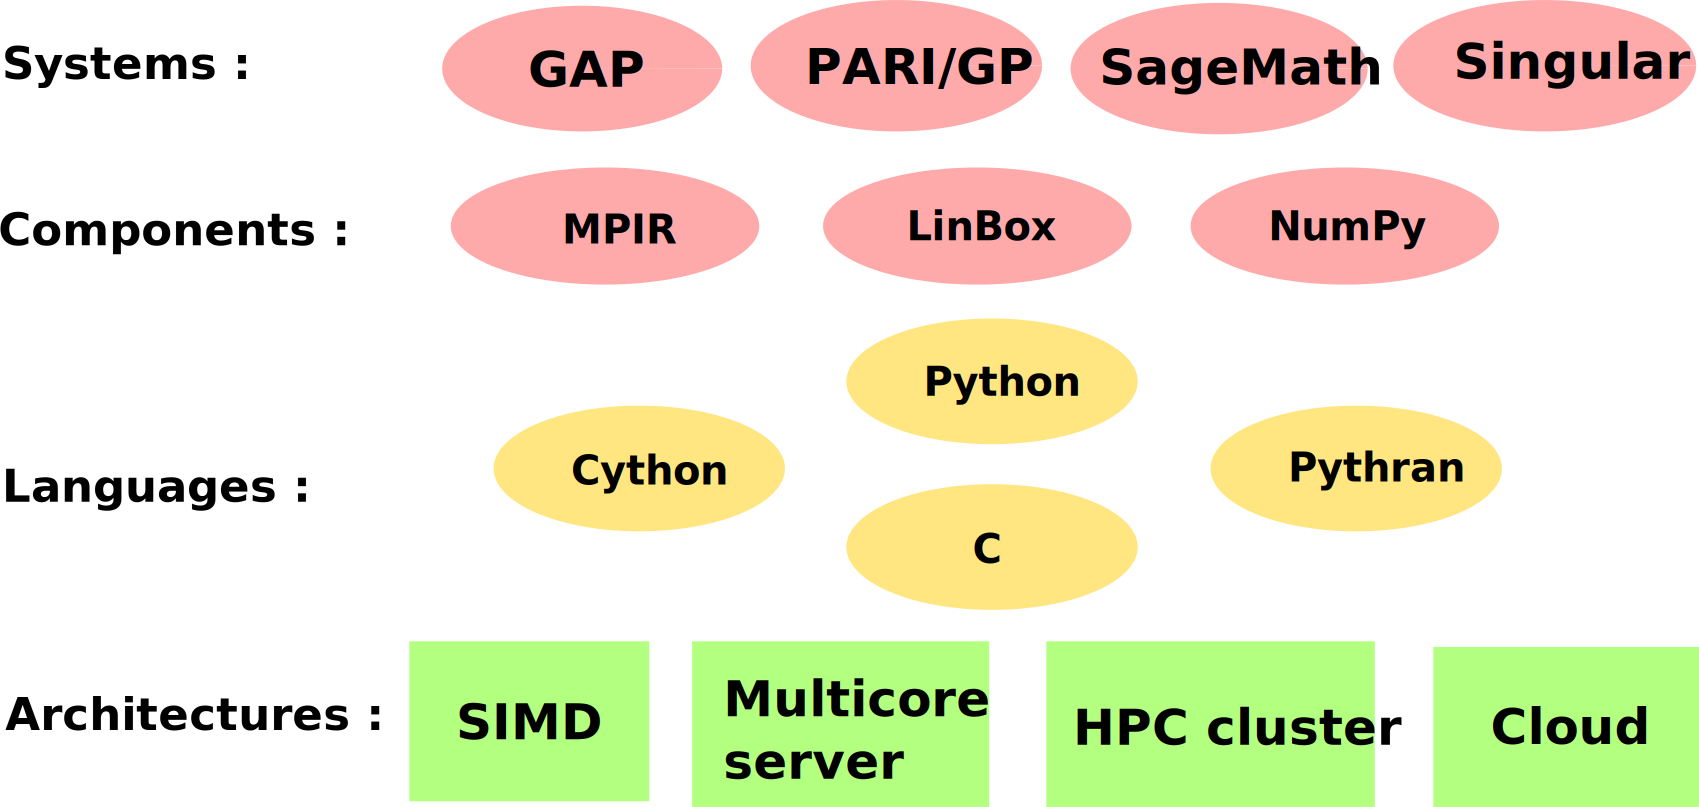
\includegraphics[width=\textwidth]{software_stack}
%%     \end{column}
%%     \begin{column}
%%       {.48\textwidth }
%%   \begin{itemize}
%%   \item High level VRE rely on the Python language
%%   \item High performance is achieved mostly by the C language\pause
%%   \item Python to C compilers: 
%%     \begin{itemize}
%%     \item Cython: general purpose
%%     \item Pythran: narrower scope, better at optimizing Numpy code (Linear
%%       algebra)
%%     \end{itemize}
%%   \end{itemize}
%%     \end{column}
%%   \end{columns}
%% \pause
%%   \begin{center}
%%     \textbf{Goal: Implement the convergence}

%%     \begin{description}
%%       \item[D5.4] Improve Pythran typing system
%%       \item[D5.2] Make Cython use Pythran backend to optimize Numpy code
%%     \end{description}
%%   \end{center}
  
%% \end{frame}
%%%%%%%%%%%%%%%%%%%%%%%%%%%%%%%%%%%%%%%
%% \begin{frame}[fragile]
%%   \frametitle{D5.2: Make Cython use Pythran backend for NumPy code}

%%   \begin{center}
%%     \includegraphics[width=.65\textwidth]{float_graph}\\
%%   \end{center}
%%   \begin{lstlisting}
%% import numpy
%% cimport numpy
%% def float_comp (numpy.ndarray[numpy.float_t, ndim=1] a,
%%                  numpy.ndarray[numpy.float_t, ndim=1] b):
%%      return numpy.sqrt(numpy.sqrt(a*a+b*b))
%% \end{lstlisting}

%% \end{frame}
%% %%%%%%%%%%%%%%%%%%%%%%%%%%%%%%%%%%%%%%%%%%%%%%%%%%%%%%%%%%%%%%%%%%
%% \begin{frame}[fragile]
%%   \frametitle{D5.2: Make Cython use Pythran backend for NumPy code}

%%   \begin{center}
%%     \includegraphics[width=.65\textwidth]{harris_graph}
%%   \end{center}
  
%%   \begin{lstlisting}[basicstyle=\tiny]
%% def harris(numpy.ndarray[numpy.float_t, ndim=2] I):
%%   cdef int m = I.shape[0]
%%   cdef int n = I.shape[1]
%%   cdef numpy.ndarray[numpy.float_t,ndim=2] dx = (I[1:,:] - I[:m-1,:])[:,1:]
%%   cdef numpy.ndarray[numpy.float_t,ndim=2] dy = (I[:,1:] - I[:,:n-1])[1:,:]
%%   cdef numpy.ndarray[numpy.float_t, ndim=2] A = dx * dx
%%   cdef numpy.ndarray[numpy.float_t, ndim=2] B = dy * dy
%%   cdef numpy.ndarray[numpy.float_t, ndim=2] C = dx * dy
%%   cdef numpy.ndarray[numpy.float_t, ndim=2] tr = A + B
%%   cdef numpy.ndarray[numpy.float_t, ndim=2] det = A * B - C * C
%%   return det - tr * tr
%% \end{lstlisting}

%% \end{frame}

%%%%%%%%%%%%%%%%%%%%%%%%%%%%%%%%%%%%%%%
%% \begin{frame}
%%       \frametitle{D5.4: Improve Pythran typing system}
%% \end{frame}

%%%%%%%%%%%%%%%%%%%%%%%%%%%%%%%%%%%%%%%
%%%%%%%%%%%%%%%%%%%%%%%%%%%%%%%%%%%%%%%
\section{Progress report on other tasks}
%%%%%%%%%%%%%%%%%%%%%%%%%%%%%%%%%%%%%%%
\subsection{T5.1: Pari}
\begin{frame}
  \frametitle{T5.1: Pari}
  \begin{block} {D5.16: Pari Suite release, fully supporting parallelization}
    \begin{itemize}
    \item D5.10 (merged in D5.16):\\ Generic parallelization engine is now mature
      (released since nov.2016). Support POSIX-threads and MPI.
    \item Current work: applying it throughout the library
      \begin{itemize}
      \item Chinese remaindering
      \item Rational linear algebra
      \item Discrete logarithm
      \item Resultants
      \item APRCL primality testing
      \end{itemize}
      
    \end{itemize}
  \end{block}
\end{frame}

%%%%%%%%%%%%%%%%%%%%%%%%%%%%%%%%%%%%%%%
\subsection{T5.2: GAP}
\begin{frame}
  \frametitle{T5.2: GAP}
  \begin{block} {D5.15: Final report of GAP development}
    \begin{itemize}
    \item 8 releases were cut integrating contributions of D3.11 and D5.15
    \item Towards an integration of HPC-GAP: main release GAP-4.9
      \begin{itemize}
      \item Build system refactoring
      \item Ability to compile in HPC-GAP compatibility mode
      \end{itemize}
    \item Work in progress:
      \begin{itemize}
      \item  Multithreaded linear algebra: at the level of the \texttt{Meataxe} library
      \item Introspection functionalities: on-the-fly optimisation decision
      \end{itemize}
    \end{itemize}
  \end{block}
\end{frame}

%%%%%%%%%%%%%%%%%%%%%%%%%%%%%%%%%%%%%%%
%% \subsection{T5.3: LinBox}
%% \begin{frame}
%%   \frametitle{T5.3 LinBox}

%%   \begin{block} {D5.14: Distributed exact linear system solving}
%% {
%%     \only<1,2>{
%%       \begin{itemize}
%%         \item 2 full time engineers
%%         \item Communication and serialization layer done
%%         \item Prototype MPI parallelization of Chinese remainder based solver.
%%       \end{itemize}
%%     }
%%     \only<3->{
%%       \begin{description}
%%       \item[Roadmap:] \
%%         \begin{itemize}
%%         \item Major refactorization of LinBox solver code under way
%%         \item Parallelization of Dixon-lifting solver
%%         \item Hybrid combination of CRT+Dixon.
%%         \item Hyrbid OpenMP-MPI implementation
%%         \end{itemize}   
%%       \end{description}
%%         \vspace{-1.4em}
%%     }
%%     \begin{columns}
%%       \begin{column} {.5\textwidth}
%%         \begin{center}
%%           \uncover<2->{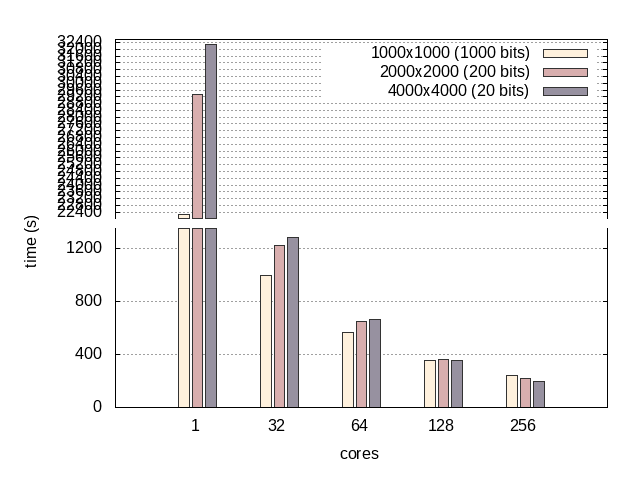
\includegraphics[width=\textwidth]{nodes_histogram}}
%%       \end{center}
%%       \end{column}
%%       \begin{column} {.45\textwidth}
%%         \begin{center}
%%           \uncover<2->{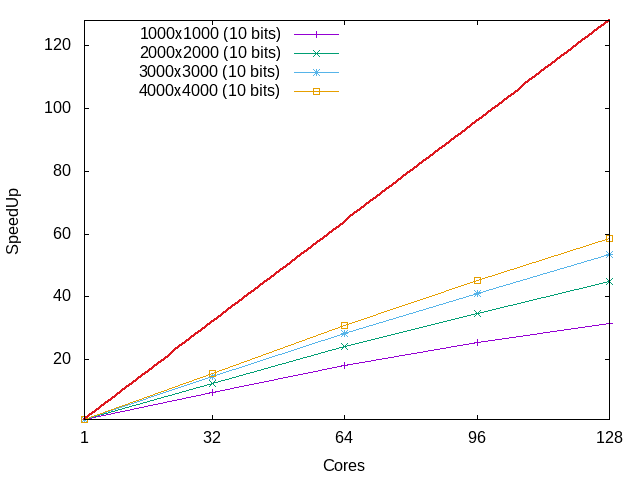
\includegraphics[width=\textwidth]{nodes_SPEEDUP}}
%%         \end{center}
%%       \end{column}
%%     \end{columns}
%% }
%%   \end{block}
%% \end{frame}
%%%%%%%%%%%%%%%%%%%%%%%%%%%%%%%%%%%%%%%%%%%%%%%%%%%%
\subsection{T5.4: Singular}
\begin{frame}
  \frametitle{T5.4 Singular}
  \begin{block}
    {D5.13: Parallel sparse polynomial multiplication}
    
    \texttt{FLINT} now supports fast sparse multivariate polynomials:
    \begin{itemize}
    \item addition, subtraction, multiplication,
    \item division, division with remainder, GCD
    \item evaluation (and partial evaluation), composition
    \end{itemize}

\uncover<2->{  \textbf{Parallelization of the (sparse) multiplication}
    \begin{columns}
      \begin{column}{.38\textwidth}
        {\footnotesize
          %% \begin{equation*}
          %%   (1 + x + y + 2z^2 + 3t^3 + 5u^5)^{21}*(1 + u + t + 2z^2 + 3y^3 + 5x^5)^{21}
          %% \end{equation*}
%          \begin{center}
            \begin{tabular}{lcccccccc}
               \toprule
               threads & time (ms) & speedup\\ \midrule
               1 & 148661 & x1.0\\
               2 & 76881 & x1.9\\ 
               3 & 54798 & x2.7\\ 
               4 & 42855 & x3.4\\ 
               5 & 37017 & x4.0\\ 
               6 & 30892 & x4.8\\ 
               7 & 28365 & x5.2\\ 
               8 & 28048 & x5.3\\
               \bottomrule
            \end{tabular}
 %         \end{center}
        }
      \end{column}
      \begin{column}{.6\textwidth}
        \uncover<3->{
          \begin{itemize}
        \item Planned improvements to the memory manager $\Rightarrow$ closer to linear scaling 
        \item Parallel division and GCD implementations are in progress.
        \item Integration into Factory/Singular remains to be done
          \end{itemize}
          }
      \end{column}
    \end{columns}
    }
   \end{block}

 \end{frame}

%% \begin{frame}
%%   \frametitle{Root clustering}
    
%%     \begin{block}{Root clustering}
%% \begin{itemize}
%%  \item Remi Imbach has implemented the new parallel root clustering algorithm of Sagraloff-Yap
%%  \item Remi will return to Kaiserslautern (from New York visiting Chee Yap) to integrate the new code in Singular
%%  \item All deliverables for Kaiserslautern are on track
%%  \end{itemize}

%%  \end{block}
%%  \end{frame}


%%%%%%%%%%%%%%%%%%%%%%%%%%%%%%%%%%%%%%%
\begin{frame}
  \frametitle{Conclusion}

  \textbf{Outcome of WorkPackage 5}
  \begin{center}
{\small
    \begin{tabular}{lccc}
    \toprule
        & Review 1 & Review 2 & Final review\\
    \midrule
    T5.1 Pari/GP & & & {\color{green} D5.16} \\
    T5.2 GAP     & & & {\color{green} D5.15} \\
    T5.3 LinBox  & & \alert{D5.12} & {\color{green} D5.14} \\
    T5.4 Singular& D5.6, D5.7 & & {\color{green} D5.13} \\
    T5.5 MPIR    & D5.5, D5.7& & \\
    T5.6 Combinatorics  & D5.1& \alert{D5.11} & \\
    T5.7 Pythran        & D5.2 & \alert{D5.11} & \\
    T5.8 SunGrid Engine & D5.3 & & \\
    \bottomrule
    
  \end{tabular}
}
  \end{center}
  
  Overall
  \begin{itemize}
  \item over 20 software relases were cut
  \item 7 research papers
  \end{itemize}
\end{frame}
  


\begin{frame}
  \frametitle{Backup Slides}

  \begin{center}
    \Large Backup Slides
  \end{center}
\end{frame}
\begin{frame}
  \frametitle{Outsourced computing security (D5.12)}

  \begin{block}{Exploratory aspect: Computation over the Cloud}
    \begin{description}
    \item[Outsourcing computation on the cloud:]\ 
      \begin{itemize}
      \item trusted lightweight client computer
      \item untrusted powerful cloud server
      \end{itemize}
      $\Rightarrow$ need for certification protocols
    \item[Multiparty computation:] \
      \begin{itemize}
      \item each player contribute with a share of the input
      \item shares must remain private
      \end{itemize}
    \end{description}
\end{block}
  \begin{block}<2->
      {Contribution}
      \begin{description}
        \item[ISSAC'17:] Linear time certificates for LU, Det., Rank Profile  matrix, etc
        \item[In submission:] Secure multiparty Strassen's algorithm
      \end{description}
  \end{block}

\end{frame}
%%%%%%%%%%%%%%%%%%%%%%%%%%%%%%%%%%%%%%%
\begin{frame}[fragile]{Exploration: Python, Cython, Pythran and Cilk (D5.8)}
  \textit{workshop: Interfacing (math) software with low level libraries}
\begin{center}
  \begin{gnuplot}[terminal=cairolatex,terminaloptions={font ",10" linewidth 2}]
  set style line 3 pt 3 pi 50 lw 4 lt rgb "blue"
  set title 'Counting descents in permutations'
  set logscale y
  set ylabel 'log time'
  set format y '%L'
  set xlabel 'n'
  set size 0.9,0.6
  set key bottom right
  plot [9:13] \
  "data_perms.txt" using 1:2 title "python" with lines lc 1, \
  "data_perms.txt" using 1:4 title "cython/pythran" with lines lc 3, \
  "data_perms.txt" using 1:6 title "cilk 1 core" with lines lc 5, \
  "data_perms.txt" using 1:7 title "cilk 8 cores" with lines lc 6
  \end{gnuplot}

\begin{itemize}
\item Python (interpreted language) slow.
\item Cython/Pythran (Python to C compilers) efficient.
\item Cilk (SIMD and multithread parallelism) very promising.
\end{itemize}
\end{center}

\end{frame}
%%%%%%%%%%%%%%%%%%%%%%%%%%%%%%%%%%%%%%%
%%%%%%%%%%%%%%%%%%%%%%%%%%%%%%%%%%%%%%%
%%%%%%%%%%%%%%%%%%%%%%%%%%%%%%%%%%%%%%%
\end{document}
